\chapter{Abkürzungsverzeichnis}

\begin{acronym}
	\acro{ssh}[SSH]{Secure Shell}	
	\acro{cwe}[CWE]{Common Weakness Enumeration}

\end{acronym}

\clearpage

\chapter{Abbildungsverzeichnis}

%\begin{figure}[H]
%	\centering
%	{\caption{Baumstruktur eines Leistungsverzeichnisses in der ORCA \ac{ava}}
%		\label{fig:LV-der-AVA}}
%	{\includegraphics[width=1\textwidth]{\figdir/orca-ava-tree}}
%\end{figure}

\begin{figure}[b!]
	{\caption{Welche IT-Projekte haben in Ihren Unternehmen die höchste Priorität}
		\label{FIG:statistic-it-projects}}
	{\includegraphics[width=1\textwidth]{figures/statistic-it-projekte.png}}
\end{figure}

\begin{figure}[b!]
	{\caption{Breakdown of software development methodologies practiced wordlwide in 2021}
		\label{FIG:devops-important}}
	{\includegraphics[width=1\textwidth]{figures/devops-important.png}}
\end{figure}

\begin{figure}[b!]
	{\caption{StackOverflow Trends von Github und Azure DevOps vom 18.06.2022}
		\label{FIG:github_azuredevops}}
	{  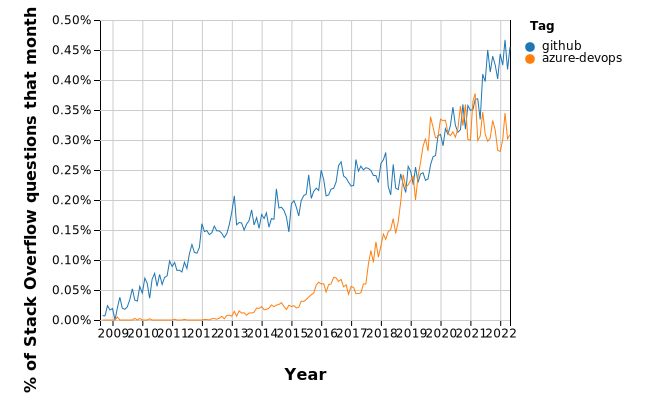
\includegraphics[width=1\textwidth]{figures/github_azuredevops.png}
	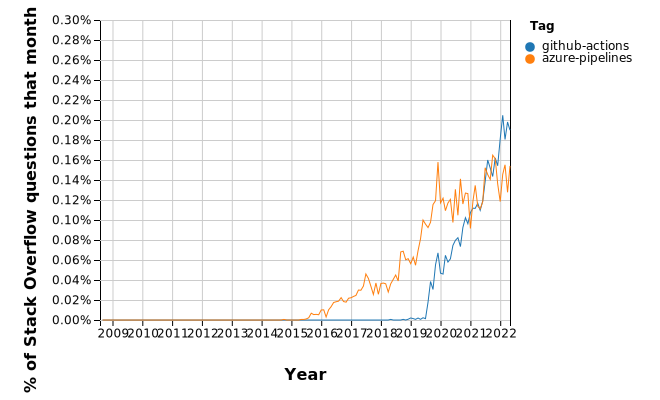
\includegraphics[width=1\textwidth]{figures/githubactions_azurepipelines.png}}
\end{figure}


%%% Local Variables: 
%%% mode: latex
%%% TeX-master: "thesis.tex"
%%% End: 
